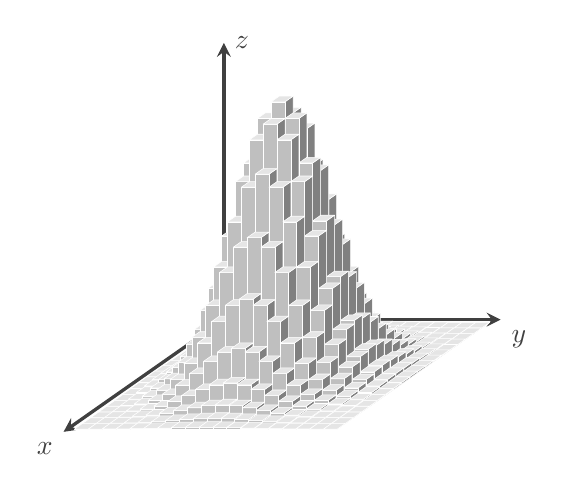
\begin{tikzpicture}[
    x=(215:2em/sqrt 2), y=(0:2em), z=(90:2em),
    declare function={ftwo(\x,\y)=5*exp(-(\x-2.5)^2-(\y-2.5)^2);}, 
  very thick, line join=round]

  % x-axis
  \draw [-stealth, black!75] (0,0,0) -- (5,0,0) node [below left] {$x$};

  % y-axis
  \draw [-stealth, black!75] (0,0,0) -- (0,5,0) node [below right] {$y$};

  % z-axis
  \draw [-stealth, black!75] (0,0,0) -- (0,0,5) node [right] {$z$};


  % Draw cubes
  \foreach \i in {1,...,19}
  \foreach \j [evaluate={\x=0.25*\i; \y=0.25*\j; \k=ftwo(\x,\y);}] in {1,...,19}{

    % x-z planes (dark) -- right
    \path [fill=black!50, draw=white,line width=0.2pt] 
    (\x-0.125, \y+0.125, 0) -- 
    (\x+0.125, \y+0.125, 0) -- 
    (\x+0.125, \y+0.125, \k) -- 
    (\x-0.125, \y+0.125, \k) -- 
    cycle;

    % z-y planes (medium) -- front
    \path [fill=black!25, draw=white,line width=0.2pt] 
    (\x+0.125, \y-0.125, 0) -- 
    (\x+0.125, \y+0.125, 0) -- 
    (\x+0.125, \y+0.125, \k) -- 
    (\x+0.125, \y-0.125, \k) -- 
    cycle;

    % x-y planes (light) -- top
    \path [fill=black!10, draw=white,line width=0.2pt] 
    (\x-0.125, \y-0.125, \k)  -- 
    (\x+0.125, \y-0.125, \k) -- 
    (\x+0.125, \y+0.125, \k) -- 
    (\x-0.125, \y+0.125, \k) -- 
    cycle;
  }

%  \foreach \i in {0,...,10}
%  \foreach \j [evaluate={\x=0.5*\i; \y=0.5*\j; \k=ftwo(\x,\y);}] in {0,...,10}{
%    \draw [black, fill=black, fill opacity=0.125, 
%    domain=0:1, samples=10, variable=\t] 
%    plot (\x+\t, \y, {ftwo(\x+\t,\y)}) -- 
%    plot (\x+1, \y+\t, {ftwo(\x+1,\y+\t)}) -- 
%    plot (\x+1-\t, \y+1, {ftwo(\x+1-\t,\y+1)}) --
%    plot (\x, \y+1-\t, {ftwo(\x,\y+1-\t)}) -- 
%    cycle;
%  }


%  % Draw functions
%  \foreach \x in {1,...,4}
%  \foreach \y in {1,...,4}{
%    \draw [black, fill=black, fill opacity=0.125, 
%    domain=0:1, samples=10, variable=\t] 
%    plot (\x-0.5+\t, \y-0.5,    {ftwo(\x-0.5+\t,\y-0.5)}) -- 
%    plot (\x+0.5,    \y-0.5+\t, {ftwo(\x+0.5,   \y-0.5+\t)}) -- 
%    plot (\x+0.5-\t, \y+0.5,    {ftwo(\x+0.5-\t,\y+0.5)}) --
%    plot (\x-0.5,    \y+0.5-\t, {ftwo(\x-0.5,   \y+0.5-\t)}) -- 
%    cycle;
%  }
\end{tikzpicture}
